\chapter{Data Sources}
\section{National Health Service Standard 43 folder}
    National Health Service Standard 43 folder or 43 folder is a collection of more than 43 folder legislate from Ministry of Public Health (MoPH). In 43 folder, there are several information about the patients such as visiting information, diagnosis from both doctor and lab test, type and amount of drug that patient receive and what type of disease that patient have. This 43 folder cover nearly all of the patient information in Thailand including immigrant worker and foreigner, however it is only include patients information from hospital that under Ministry of Public Health (MoPH) exclude Bangkok. This is because hospital in Bangkok is under the management of Bangkok Administration.
    
\section{Data Schema}
    In our system, we do not need all 43 folders to process the data. We only need the following folders.
    
    % Thai officer position in English
    % http://wangkapee.uttaradit.police.go.th/InPos.html
    % https://web.facebook.com/Ed1BO/posts/494806177306805?_rdr
    
    \subsection{PERSON}
        In this folder, it stores the data of patient who does not live in hospital's region or patient who lives in hospital's region but his/her household registration is not in hospital's region. It is consist of hospcode(hospital code), CID (Citicen ID), PID (Patient ID), name, birth date and etc. For complete detail of PERSON folder you can look at \ref{person_folder}.
    
    \subsection{ADDRESS}
        In this folder, it stores the address of a patient who lives outside responsible district or patient who live inside responsible district but his/her household registration is outside the district.For complete detail of ADDRESS folder you can look at \ref{address_folder}.
        
        % % http://www.dailyenglish.in.th/english-address/
\begin{enumerate}
  \item HOSPCODE: Hospital code that is defined by the Bureau of Policy and Strategy (under Ministry of Public Health). 
  \item PID: Person identification number who registers in the hospital. This is used for identifying the person in other folders (the range of digits can be between 1 to 15 and generated by program).
  \item ADDRESSTYPE: Type of address. 1 = Address in household registration, 2 = Address that is reachable by contact.
  \item HOUSE\_ID: House identification number that is assigned by Department of Provincial Administration (under Ministry of Interior).
  \item HOUSE\_TYPE: The type of residence. 1 = Detached House or Semi Detached House, 2 = Townhouse, 3 = Condominium, 4 = Apartment or Dormitory, 5 = Labor Home-stay, 8 = etc, 9 = unknown.
  \item ROOMNO: The room number if HOUSE\_TYPE is an apartment or dormitory.
  \item CONDO: The name of building, condominium, or dormitory.
  \item HOUSENO: Street number
  \item SOISUB: Sub lane
  \item SOIMAIN: Lane
  \item ROAD: The road's name
  \item VILLANAME: The village's name
  \item VILLAGE: The village number. Use 99 if unknown.
  \item TAMBON: Sub district code that is defined by Department of Provincial (under Ministry of Interior). Use 99 if unknown.
  \item AMPUR: District code that is defined by Department of Provincial (under Ministry of Interior). Use 99 if unknown.
  \item CHANGWAT: Province code that is defined by Department of Provincial (under Ministry of Interior). Use 99 if unknown.
  \item TELEPHONE: Telephone number
  \item MOBILE: Mobile phone number
  \item D\_UPDATE: The date in which this folder has been modified. The format is YYYYMMDDHHMMSS and the year format is CE.
\end{enumerate}
        
    \subsection{DEATH}
        This folder stores the history of death of citizens who lived in the responsible district and patient. It consists of death date, disease code and etc.For complete detail of DEATH folder you can look at \ref{death_folder}.
        % \begin{enumerate}
  \item HOSPCODE: Hospital code that is defined by the Bureau of Policy and Strategy (under Ministry of Public Health). 
  \item PID: Person identification number who registers in the hospital. This is used for identifying the person in other folders (the range of digits can be between 1 to 15 and generated by program).
  \item HOSPDEATH: Hospital code in a case that patient died in the hospital. If they can not determine which hospital, mark it as 00000.
  \item AN: Inpatient number in which the patient died in the hospital
  \item SEQ: The order of the service that be provided by the program. the number is unique, and sort by order of SEQ in each service (visit).
  \item DDEATH: Date that patient died. The format is YYYYMMDD and the year format is CE.
  \item CDEATH\_A: Disease code A according to Certificate of Death. 
  \item CDEATH\_B: Disease code B according to Certificate of Death.
  \item CDEATH\_C: Disease code C according to Certificate of Death.
  \item CDEATH\_D: Disease code D according to Certificate of Death.
  \item ODISEASE: Other disease code or other factor of death according to Certificate of Death.
  \item CDEATH: Cause of death according to the Certificate of Death.
  \item PREGDEATH: 1 = Death in pregnancy, 2 = Maternal Death
  \item PDEATH: The place where patient died. 1 = In hospital, 2 = Outside hospital.
  \item PROVIDER: Doctor of patient number that is generated by the program. It must be unique within the same hospital.
  \item D\_UPDATE: The date in which this folder has been modified. The format is YYYYMMDDHHMMSS and the year format is CE.
\end{enumerate}
        
    \subsection{SERVICE}
        In this folder, it contains the data about the history of the service that be provided to the patient who come to receive and also provide the service outside the hospital area.For complete detail of SERVICE folder you can look at \ref{service_folder}.
        % \begin{enumerate}
  \item HOSPCODE: Hospital code that is defined by the Bureau of Policy and Strategy (under Ministry of Public Health). 
  \item PID: Person identification number who registers in the hospital. This is used for identifying the person in other folders (the range of digits can be between 1 to 15 and generated by program).
  \item HN: Outpatient number that receive when the patient come to receive the service (the range of digits can be between 1 to 15)
  \item SEQ: The order of the service that be provided by the program. the number is unique, and sort by order of SEQ in each service (visit).
  \item DATE\_SERV: The date receiving the service. Defining format as year (in CE format), month and date  by order(YYYYMMDD). NOTE that in case have to record previous data, have to change the date to the date that receive the service.
  \item TIME\_SERV: Time hospital provide a service and defining format as  hour, minute, and second as (HHMMSS)  
  \item LOCATION: The area of the patient. There are two type of it which are (1) means area of responsibility and (2) means area of irresponsibility
  \item INTIME: The time that patient come and receive the service. There are two type of it which are (1) means in office hours and (2) means out of the office hours.
  \item INSTYPE: The right to medical care code that the patient use each visit.
%   ประเภทสิทธิการรักษา
%   รหัสสิทธิมาตรฐาน ที่ใชในการมารับบริการ
  \item INSID: The id number of the card of the right to medical care according to the type of the right to medical care.
%   หมายเลขของบัตร ตามประเภทสิทธิการรักษา
  \item MAIN: The standard code that come from Bureau of Policy and Strategy in order to describe the main service place.
  \item TYPEIN: It is a types of service that patient come to receive the service. There are four main types which are (1) means the patient come to receive the service by themselves, (2) means the patient come to receive the service according to the appointment, (3) means the patient that be transferred from one to other hospital, and (4) means the patient that be transferred from EMS.
  \item REFERINHOSP: The code of the hospital that send the patient to here. 
  \item CAUSEIN: The reason that transfer the patient to receive the service here. There are five main types which are (1) means to diagnose and treat, (2) means to diagnose, (3) means to treat and recover, (4) means to receive the service that close to their home, and (5) means to receive the service according to the patient's need.
  \item CHIEFCOMP: The important symptoms that patient has to come to use the service.
  \item SERVPLACE: The place that receive the service. There are 2 types which are (1) means in the service place and (2) means outside the service place
  \item BTEMP: The body temperature that measure when the patient come in. It should be in Celsius with two digits and one decimal place.
  \item SBP: Systolic pressure that first given. It should be three or less than three digits. Note that if cannot measure, not need to record
  \item DBP: Diastolic pressure that first given. It should be three or less than three digits. Note that if cannot measure, not need to record
  \item PR: Heart rate per minute. It should be three or less than three digits.
  \item RP: Breath rate per minute. It should be three or less than three digits.
  \item TYPEOUT: The status of patient after they are done receiving the service. There are nine main types which are (1) means receive drug and can go back home, (2) means receiving as Inpatient, (3) means the patient is sent to other hospital, (4) mean dead, (5) means dead before receiving the service at hospital, (6) means dead during the transfer process to other hospital, (7) means decline to treat. (8) means escape. (9) mean receive the service without diagnosis result.
  \item REFEROUTHOSP: The hospital code that transfer the patient to have a treatment.
  \item CAUSEOUT: The reason to transfer the patient to receive the service. There are five main types which are (1) means to diagnose and treat, (2) means to diagnose, (3) means to treat and recover, (4) means to receive the service that close to their home, and (5) means to receive the service according to the patient's need.
  \item COST: Total cost of treatment including drug, medical supplies, treatment. It should be eight digits and two decimal place. If it is no price, put 0.00.
  \item PRICE:Total price of treatment including drug, medical supplies, treatment. It should be eight digits and two decimal place. If it is no price, put 0.00.
  \item PAYPRICE: Total price that patient have to pay since it is the expenses that cannot be issued to the government. . It should be eight digits and two decimal place. If it is no price, put 0.00.
  \item ACTUALPAY: Total price that the patient have to pay. It should be eight digits and two decimal place. If it is no price, put 0.00.
  \item D\_UPDATE: The date in which this folder has been modified. The format is YYYYMMDDHHMMSS and the year format is CE.
  
  
\end{enumerate}
        
    \subsection{DIAGNOSIS\_OPD}
        In this folder, it contains the diagnosis of the Out-patient and patient who come to receive the service. For complete detail of DIAGNOSIS\_OPD folder you can look at \ref{diagnosis_opd_folder}.
        % \begin{enumerate}
  \item HOSPCODE: Hospital code that is defined by the Bureau of Policy and Strategy (under Ministry of Public Health). 
  \item PID: Person identification number who registers in the hospital. This is used for identifying the person in other folders (the range of digits can be between 1 to 15 and generated by program).
  \item SEQ: The order of the service that be provided by the program. the number is unique, and sort by order of SEQ in each service (visit).
  \item DATE\_SERV: The date receiving the service. Defining format as year(Anno Domini(AD)), month and date  by order(YYYYMMDD). NOTE that in case have to record previous data, have to change the date to the date that receive the service.
  \item DIAGTYPE: Type of diagnosis. 1 = Principle DX, 2 = Co-Morbidity, 3 = Complication, 4 = other, 5 = External Cause, 6 = Additional Code, 7 = Morphology Code. In case of out-patient, use only 1, 4, 5 or 7.
  \item DIAGCODE: Disease code in ICD-10-TM
  \item CLINIC: Ward code that is defined by the Bureau of Policy and Strategy (under Ministry of Public Health).
  \item PROVIDER: Doctor of patient number that is generated by the program. It must be unique within the same hospital.
  \item D\_UPDATE: The date in which this folder has been modified. The format is YYYYMMDDHHMMSS and the year format is CE.
\end{enumerate}
        
    \subsection{DRUG\_OPD}
        In this folder, it contains the data that providing drug for Out-patient and patient who come to receive the service. For complete detail of DRUG\_OPD folder you can look at \ref{drug_opd_folder}.
        % \begin{enumerate}
  \item HOSPCODE: Hospital code that is defined by the Bureau of Policy and Strategy (under Ministry of Public Health). 
  \item PID: Person identification number who registers in the hospital. This is used for identifying the person in other folders (the range of digits can be between 1 to 15 and generated by program).
  \item SEQ: The order of the service that be provided by the program. the number is unique, and sort by order of SEQ in each service (visit). 
  \item DATE\_SERV: The date that receive the service Defining format as year(format CE), month and date by order (YYYYMMDD). NOTE that in case have to record previous data, have to change the date to the date that receive the service.
  \item CLINIC: Service department code according to Bureau of Policy and Strategy
  \item DIDSTD: The standard medicine code that is set in 24 digits and the medicine code of hospital in case that they do not have The standard medicine code.
  \item DNAME: Name of the drug
  \item AMOUNT: The amount of medicine that be provided and it has to be in 12 digit(no more than 12 digits)
  \item UNIT: Unit of medicine. It is the standard code that come from Bureau of Policy and Strategy  
  \item UNIT\_PACKING: Packing size per unit that is counting in Field UNIT  
  \item DRUGPRICE: The price of medicine that sell to the patient
  \item DRUGCOST: The buying price or the price of medicine that be received from hospital  
  \item PROVIDER: Service person number that generated from the program and the number is unique in each hospital.
  \item D\_UPDATE: The date in which this folder has been modified. The format is YYYYMMDDHHMMSS and the year format is CE.
\end{enumerate}











        
    \subsection{LABFU}
        In this folder, it stores the  lab result that come from the lab of patient who have diseases. For complete detail of LABFU folder you can look at \ref{labfu_folder}.
        % \begin{enumerate}
  \item HOSPCODE: Hospital code that is defined by the Bureau of Policy and Strategy (under Ministry of Public Health). 
  \item PID: Person identification number who registers in the hospital. This is used for identifying the person in other folders (the range of digits can be between 1 to 15 and generated by program).
  \item SEQ: The order of the service that be provided by the program. the number is unique, and sort by order of SEQ in each service (visit). 
  \item DATE\_SERV: The date receiving the service. Defining format as year(format CE), month and date by order (YYYYMMDD). NOTE that in case have to record previous data, have to change the date to the date that receive the service.
%   Do we need to include ICD-10-TM??
  \item LABTEST: ICD-10-TM Laboratory Test Code
  \item LABRESULT: Results of laboratory tests (2-digit decimal point)
  \item D\_UPDATE:  The date in which this folder has been modified. The format is YYYYMMDDHHMMSS and the year format is CE.
\end{enumerate}


    \subsection{ADMISSION}
        In this folder, it stores the history record of patient's admission of the hospital. For complete detail of ADMISSION folder you can look at \ref{admission_folder}.
        % \begin{enumerate}
  \item HOSPCODE: Hospital code that is defined by the Bureau of Policy and Strategy (under Ministry of Public Health). 
  \item PID: Person identification number who registers in the hospital. This is used for identifying the person in other folders (the range of digits can be between 1 to 15 and generated by program).
  \item SEQ: The order of the service that be provided by the program. the number is unique, and sort by order of SEQ in each service (visit).
  \item AN: Inpatient number
  \item DATETIME\_ADMIT: Date in which the hospital admits the patient. The format is YYYYMMDDHHMMSS and the year format is CE.
  \item WARDADMIT: The ward code that admits the patients that is defined by the Bureau of Policy and Strategy (under Ministry of Public Health).
  \item INSTYPE: The right to medical care code that the patient use each visit.
  \item TYPEIN: It is a types of service that patient come to receive the service. There are four main types which are (1) means the patient come to receive the service by themselves, (2) means the patient come to receive the service according to the appointment, (3) means the patient that be transferred from one to other hospital, and (4) means the patient that be transferred from EMS.
  \item REFERINHOSP: Hospital code that refers the patient.
  \item CAUSEIN: The reason that transfer the patient to receive the service here. There are five main types which are (1) means to diagnose and treat, (2) means to diagnose, (3) means to treat and recover, (4) means to receive the service that close to their home, and (5) means to receive the service according to the patient's need.
  \item ADMITWEIGHT: Patient's kilogram weight with 1 decimal.
  \item ADMITHEIGHT: Patient's centimeter height.
  \item DATETIME\_DISCH: Date and time that the hospital discharges the patient. The format is YYYYMMDDHHMMSS and the year format is CE.
  \item WARDDISCH: The ward code that discharges the patients. The code is defined by the Bureau of Policy and Strategy (under Ministry of Public Health).
  \item DISCHSTATUS: The discharge status of the patient.
  \item DISCHTYPE: The discharge type of patient.
  \item REFEROUTHOSP: The hospital code that transfer the patient to have a treatment.
  \item CAUSEOUT: The reason to transfer the patient to receive the service. There are five main types which are (1) means to diagnose and treat, (2) means to diagnose, (3) means to treat and recover, (4) means to receive the service that close to their home, and (5) means to receive the service according to the patient's need.
  \item COST: The cost of the service with 2 decimals which include medicine, medical supplies, and medical service.
  \item PRICE: The price of the service with 2 decimals which include, medicine, medical supplies, and medical service.
  \item PAYPRICE: The price with 2 decimals that patient needs to pay since it is the expenses that can not be issued to the government.
  \item ACTUALPAY: The actual price that the patient pays.
  \item PROVIDER: Doctor of patient number that is generated by the program. It must be unique within the same hospital.
  \item D\_UPDATE: The date in which this folder has been modified. The format is YYYYMMDDHHMMSS and the year format is CE.
  \item DRG: DRG group which comes from the patient's information by Grouper program according to the Government Gazette. It has 5 digits.
  \item RW: The relative weight of the in-patient. It comes from calculation of Grouper program according to the Government Gazette. It contains 4 decimals and the digits can not be more than 6. If it is unknown, mark it as 0.0000
  \item ADJRW: The relative weight that has been adjusted.
  \item ERROR: Error code about in-patient information. It comes from calculation of Grouper program according to Government Gazette.
  \item WARNING: Warning code about in-patient information. It comes from the calculation of Grouper program according to Government Gazette.
  \item ACTLOS: Patient's amount of sleep in hospital in which the value comes from the calculation of Grouper program according to the Government Gazette.
  \item GROUPER\_VERSION: The version number of Grouper program.
\end{enumerate}

    \subsection{DIAGNOSIS\_IPD}
        In this folder, it stores the data of diagnosis for In-patient. For complete detail of DIAGNOSIS\_IPD folder you can look at \ref{diagnosis_ipd_folder}.
        % \begin{enumerate}
  \item HOSPCODE: Hospital code that is defined by the Bureau of Policy and Strategy (under Ministry of Public Health). 
  \item PID: Person identification number who registers in the hospital. This is used for identifying the person in other folders (the range of digits can be between 1 to 15 and generated by program).
  \item AN: Inpatient number
  \item DATETIME\_ADMIT: Date in which the hospital admits the patient. The format is YYYYMMDDHHMMSS and the year format is CE.
  \item WARDDIAG: The ward code that admits the patients that is defined by the Bureau of Policy and Strategy (under Ministry of Public Health).
  \item DIAGTYPE: Type of diagnosis. 1 = Principle DX, 2 = Co-Morbidity, 3 = Complication, 4 = other, 5 = External Cause, 6 = Additional Code, 7 = Morphology Code.
  \item DIAGCODE: Disease code in ICD-10-TM
  \item PROVIDER: Doctor of patient number that is generated by the program. It must be unique within the same hospital.
  \item D\_UPDATE: The date in which this folder has been modified. The format is YYYYMMDDHHMMSS and the year format is CE.
\end{enumerate}
    
    \subsection{DRUG\_IPD}
        In this folder, it contains the data that providing drug for In-patient. It contain types of drug and how much drug that have been use.For complete detail of DRUG\_IPD folder you can look at \ref{drug_ipd_folder}.
        % \begin{enumerate}
  \item HOSPCODE: Hospital code that is defined by the Bureau of Policy and Strategy (under Ministry of Public Health). 
  \item PID: Person identification number who registers in the hospital. This is used for identifying the person in other folders (the range of digits can be between 1 to 15 and generated by program).
  \item AN: AN is Inpatient number
  \item DATETIME\_ADMIT: Date, month, year and the time that hospital receive the patient. The year format is CE.(YYYYMMDDHHMMSS)
  \item WARDSTAY: The code of the area that receive the patient according to Bureau of Policy and Strategy
  \item TYPEDRUG: Dispensing type can be categorized into two types which are (1) means medicine that provide to the patient who is recovering at hospital and (2) means medicine that provide to the patient who is recovering at home
  \item DIDSTD: The standard medicine code that is set in 24 digits and the medicine code of hospital in case that they do not have The standard medicine code.
  \item DNAME: Name of the drug
  \item DATESTART: The beginning date that give medicine to patient who is recovering at hospital. Defining format as (YYYYMMDD). YYYY = year format is CE., MM = month and it has to be in two digits (01-12), DD = date and it has to be in two digits (01-31)1-31
  \item DATEFINISH: The ending date that stop giving medicine to patient who is recovering at hospital. Defining format in order of (YYYYMMDD) where year format is CE.
  \item AMOUNT: The amount of medicine that be provided and it has to be in 12 digit(no more than 12 digits)  
  \item UNIT: Unit of medicine. It is the standard code that come from Bureau of Policy and Strategy  
  \item UNIT\_PACKING: Packing size per unit that is counting in Field UNIT  
  \item DRUGPRICE: The price of medicine that sell to the patient
  \item DRUGCOST: The buying price or the price of medicine that be received from hospital  
  \item PROVIDER: Service person number that generated from the program and the number is unique in each hospital.
  \item D\_UPDATE: The date in which this folder has been modified. The format is YYYYMMDDHHMMSS and the year format is CE.
\end{enumerate}
        
\section{43 Health Folder Relationship}
    As we mention above that we don't need information from all 43 folder. Therefore we filter out the floder that relevant to our big problem which is include PERSON, ADDRESS, SERVICE, ADMISSION, LABFU, DEATH, DIAGNOSIS\_OPD, DIAGNOSIS\_IPD, DRUG\_OPD and DRUG\_IPD. Relationship between those folder was impact by the patient condition. Firstly, if there is a new patient come into the system then that patient personal information will go to PERSON and ADDRESS folder. Next if the patient come to only get diagnosis result and receive drug then go back home then those information will send to SERVICE, DIAGNOSIS\_OPD and DRUG\_OPD folder. Third, if patient need to admit to the hospital then those information will go to following folder; SERVICE, ADMISSION, DIAGNOSIS\_IPD, DRUG\_IPD folder. Fourth, if patient come to have lab test then the information will go to SERVICE and LABFU folder. Lastly, if there are any patient who die in the hospital area then those information will go to DEATH folder.
        \FloatBarrier
        \begin{figure}[h!]
            \centering
                % can use width=\linewidth
        		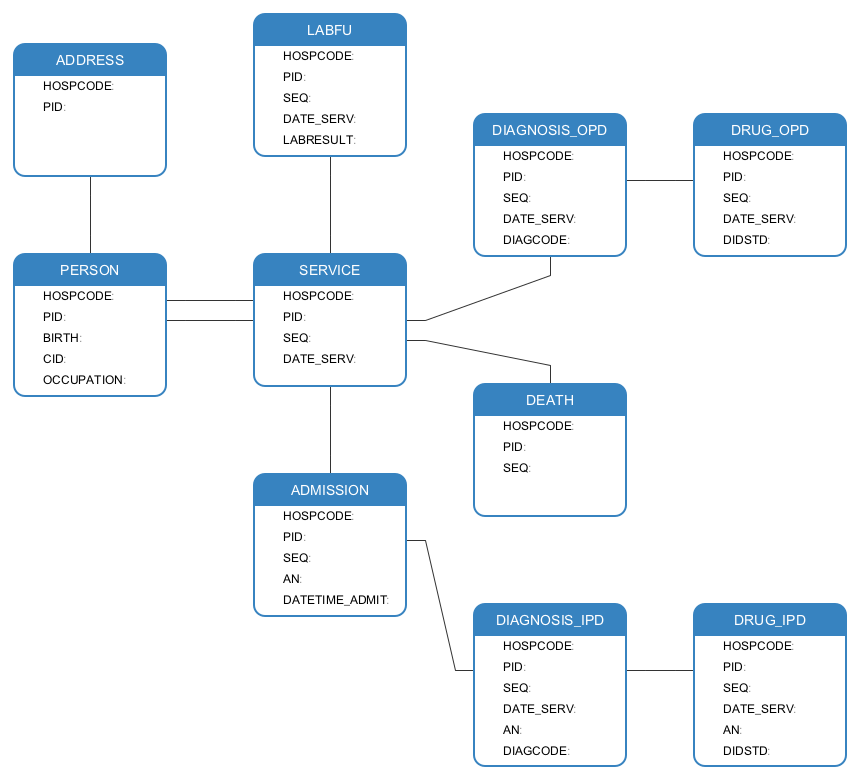
\includegraphics[width=\linewidth]{images/chapter-04/43-folders-relationship.png}
            	\caption{43 Folder Relationship}
        		\label{figure-43-folder-relationship}
        \end{figure}
        \FloatBarrier

\section{How the Data Flow} \label{section:how-the-data-flow}
    % (2014 up to now) 946GB++
    % Intro
    To begin with, there are four main areas that the data goes through which are Hospital, Provincial Public Health Office(PHO), Ministry of Public Health-ICT(MoPH-ICT), and Bureau of Policy and Strategy(BPS) as shown in figure \ref{fig_data_flow1}. First of all, the data start at the hospital area when staff have to record their patient information when patient walk in to the hospital and check  by using the program that they have in order to record. This step is shown in number one in figure \ref{fig_data_flow1}. After finish the first phase, hospital have to send the data or we known as "43 file" to PHO in less than or equal 1 month. It mean that staff at hospital have to send the data to PHO every month as it shown in number two in figure \ref{fig_data_flow3}. Then the staff at PHO will verify the data that is sent by hospital, and then they will report the data  that have error back to hospital in order to review and fix the data. Every day the staff at PHO have to send the summary data such as record of patient that visit to hospital to MoPH-ICT. Also, PHO have to send 43-file to MoPH-ICT in every 15 days as it shown in figure \ref{fig_data_flow3}, then the staff of MoPH-ICT have to update data that they receive from PHO in a day. After that, the data will be updated to the system as show in number 4 in figure \ref{fig_data_flow4}, then the system will use that data to analysis and visualize the report to web-application as it shown in number 4 in figure \ref{fig_data_flow4}. In addition, the last area is BPS where the system will get the dead data that we are missing. The data that come in to the system do not cover all dead data, it include only dead data that patient who die in hospital, but it is not include the patient who die outside the hospital, so we have to make a request to get the missing dead data at BPS. However, we can not conclude yet that how we will get the data from BPS, it is still in the processing of discussion to find the way to get the dead data.

    \FloatBarrier
        \begin{figure}[h!]
            \centering
                % can use width=\linewidth
            	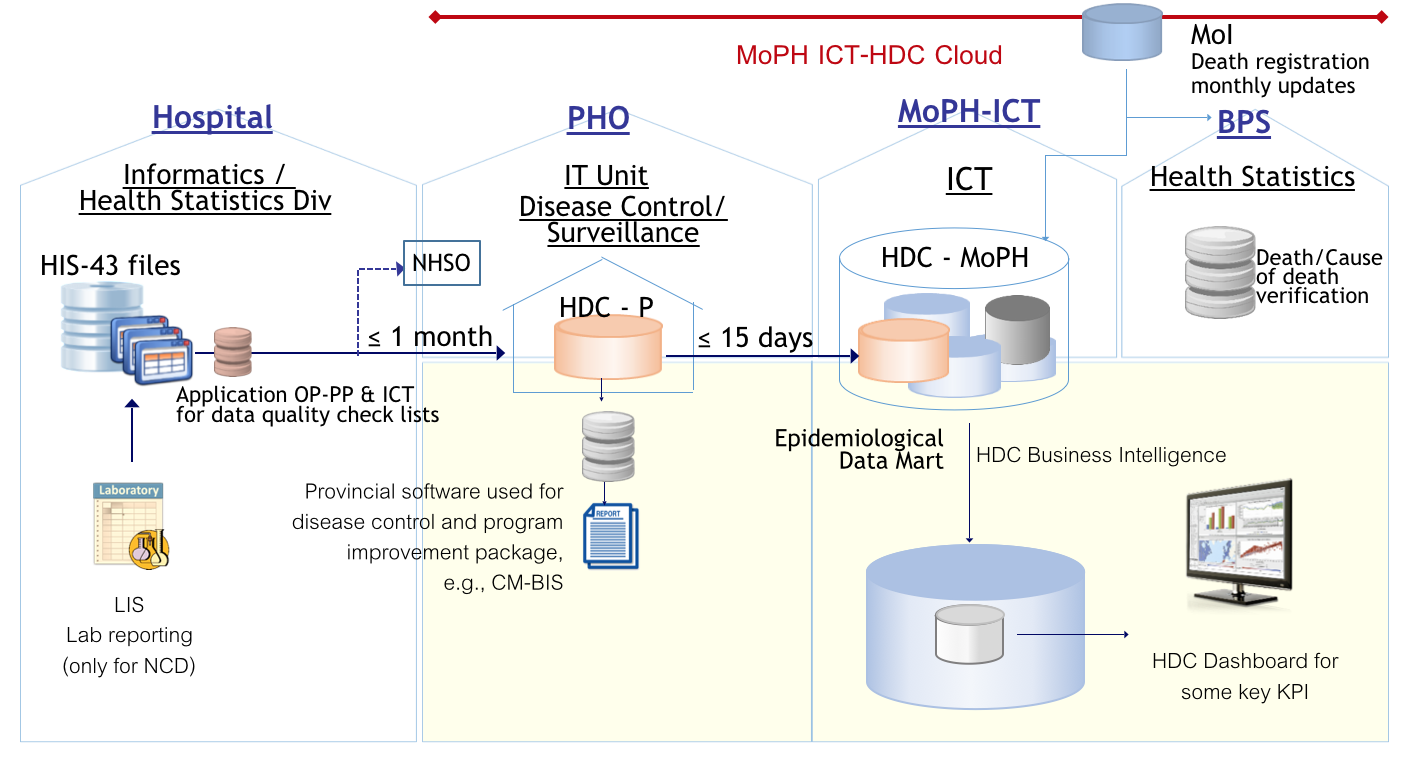
\includegraphics[width=9cm]{images/chapter-04/data_flow1.png}
            	\caption{Data Flow 1}
            	\label{fig_data_flow1}
        \end{figure}
    \FloatBarrier
    \FloatBarrier
        \begin{figure}[h!]
            \centering
                % can use width=\linewidth
            	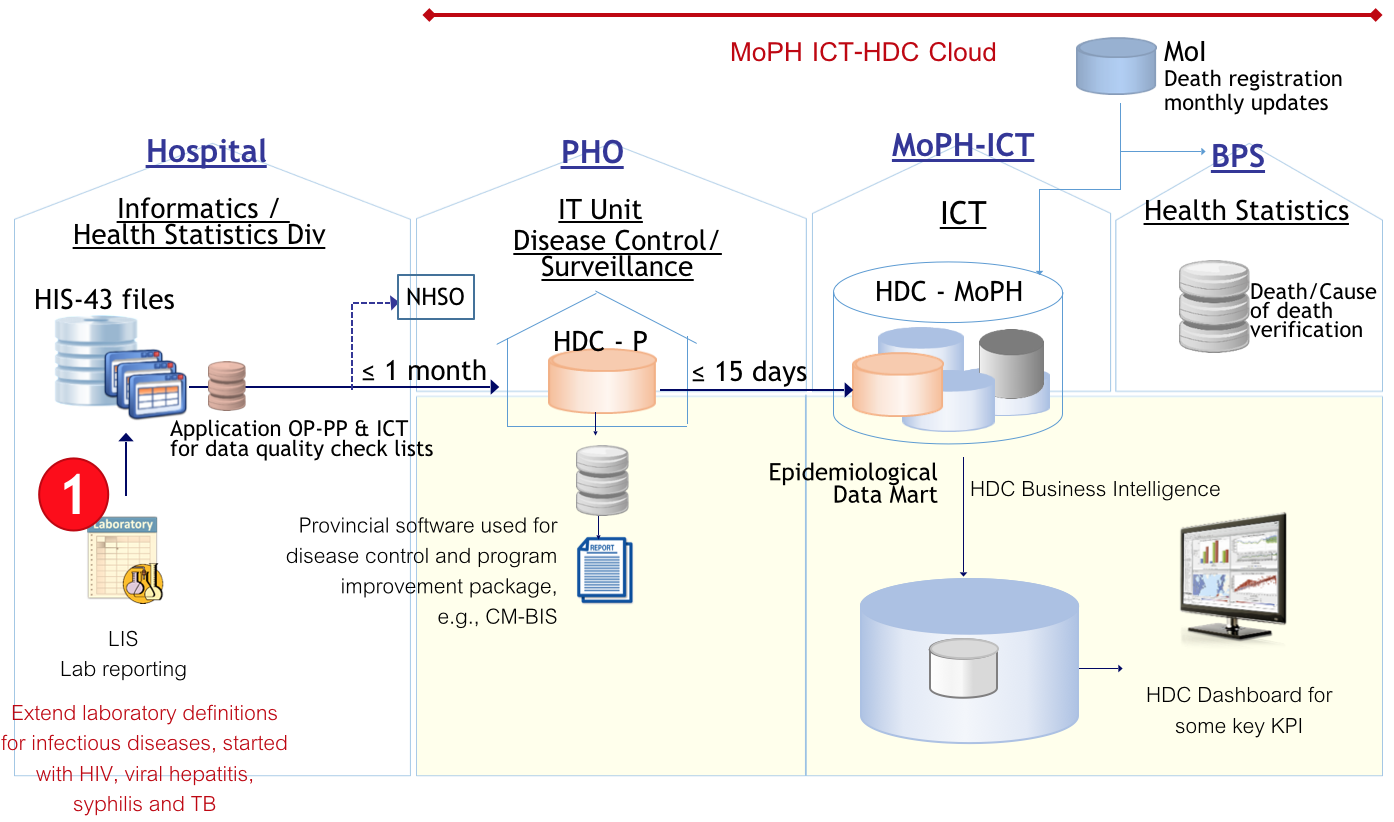
\includegraphics[width=9cm]{images/chapter-04/data_flow2.png}
            	\caption{Data Flow 2}
            	\label{fig_data_flow2}
        \end{figure}
    \FloatBarrier
    \FloatBarrier
        \begin{figure}[h!]
            \centering
                % can use width=\linewidth
            	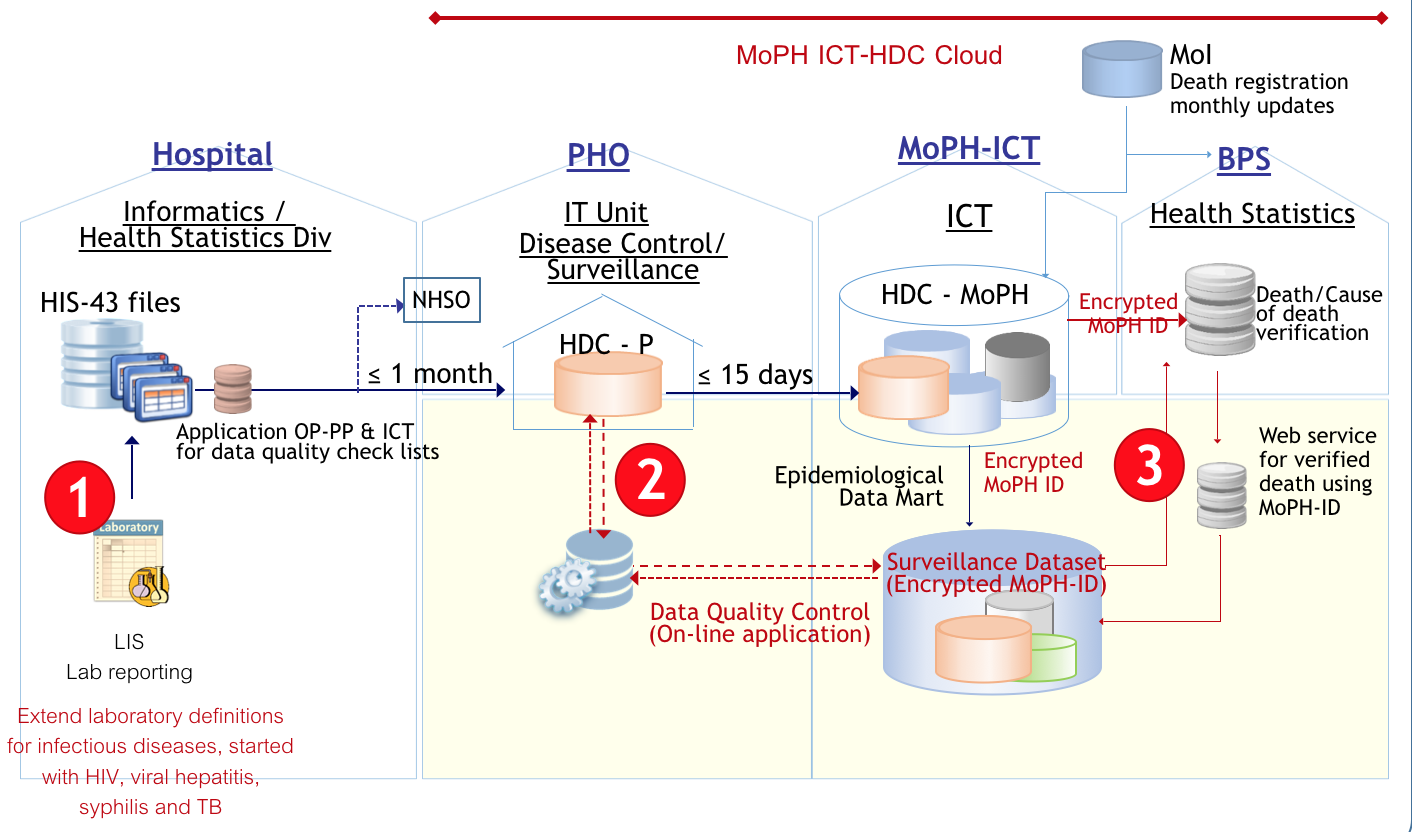
\includegraphics[width=9cm]{images/chapter-04/data_flow3.png}
            	\caption{Data Flow 3}
            	\label{fig_data_flow3}
        \end{figure}
    \FloatBarrier
    \FloatBarrier
        \begin{figure}[h!]
            \centering
                % can use width=\linewidth
            	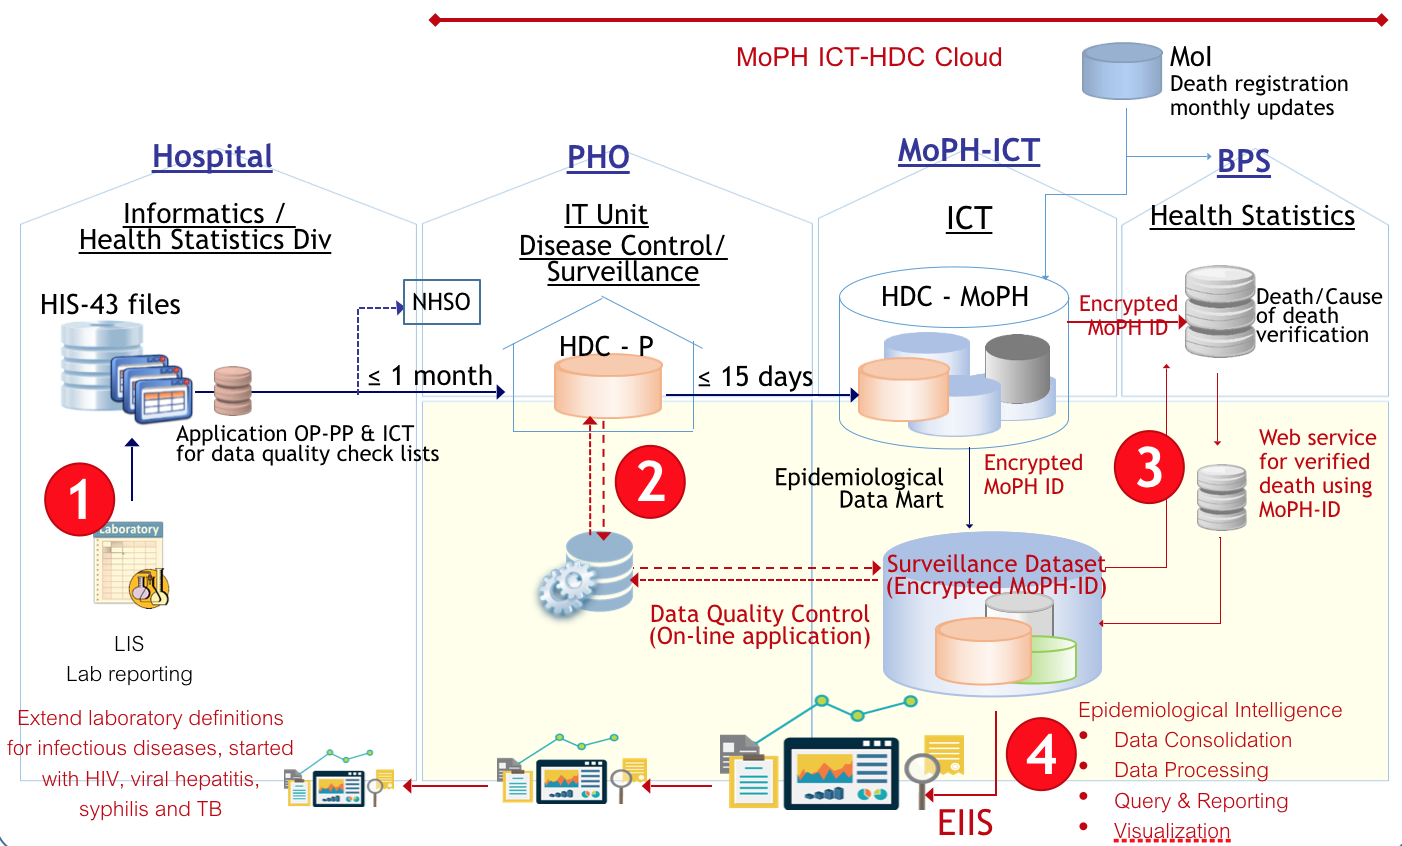
\includegraphics[width=9cm]{images/chapter-04/data_flow4.png}
            	\caption{Data Flow 4}
            	\label{fig_data_flow4}
        \end{figure}
    \FloatBarrier
    
% death แจ้งผู้ใหญ่บ้าน